\section{摘要}
本文提出了一种新的时间序列预测方法。
在这篇文章中,我们提出了一种全新的时间序列预测技术。众所周知,时间序列数据在
许多科学和工程领域中都有广泛的应用。解读这些数据,并对其进行有效预测,一直是
机器学习领域中的一个核心问题。我们的研究团队开发了一种新颖的方法,该方法采用了
基于Transformer的机器学习模型
,目的就是提高我们对时间序列数据的预测精度。这个方法利用自注意力机制,从时间
序列数据中学习并理解其内在的复杂模式和动态变化。值得一提的是,这种预测框架具有很
高的通用性。不论是对单变量还是多变量的时间序列数据,或者是时间序列嵌入,都可
以应用这个框架进行预测。
为了验证这个新方法的有效性,我们进行了一项案例研究,选择了流感样似症(ILI)的
预测作为案例。研究结果表明,我们的方法所产生的预测结果与当前最先进的预测技术相比
,具有极高的竞争力。
\section{引言}
季节性流感的全球流行给我们的健康和经济带来了沉重的压力。据统计,全球每年因流
感致死的人数惊人地高达291,000至646,000人。在美国,疾病控制与预防中心(CDC)
会利用他们的监测网络,每周发布一次有关流感症状的报告。虽然这种方式在追踪疾病流
行的规模上发挥了重要作用,但由于数据收集和整理的时间,这些报告通常至少会有一周
的延迟。因此,预测流感症状的活动就显得尤为重要,它能够帮助我们实时监测疾病的
发展,以及为公共卫生机构分配资源、制定应对潜在大流行的计划和准备提供重要参考。

为了预测这些流感症状的时间序列数据,科学家们已经开发了各式各样的方法,从机械模
型到统计和机器学习的方法,应有尽有。其中,机械模型主要是基于对疾病传播动态的
理解。例如,像SIR这样的隔室方法就是常用的模拟疾病传播动态的工具。

统计和机器学习的方法则是借助真实数据去学习和掌握趋势与模式。其中,有一些广为流
传的方法,例如自回归(AR)、自回归滑动平均(ARMA)以及自回归积分滑动平均
(ARIMA)。除此之外,一些基于卷积和循环神经网络的深度学习方法也被开发出来
,用于模拟流感症状数据。这些序列对齐的模型自然是处理时间序列数据的首选。然而,
循环神经网络中存在梯度消失和梯度爆炸的问题,而卷积滤波器也有其局限性,这些都使得
这些方法在处理序列数据中的长期和复杂关系时有所不足。

在我们的这项研究中,我们基于Transformer架构开发了一种新颖的时间序列预测方法
。与序列对齐模型不同,Transformer并不是按照顺序处理数据,而是一次性处理整个
数据序列,并利用自我注意力机制去学习序列中的依赖关系。因此,基于Transformer
的模型具有一定的潜力,能够处理那些对于序列模型具有挑战性的复杂时间序列数据。我们以流
感症状预测为案例,展示了基于Transformer的模型在时间序列预测任务上的应用,
结果表明,这种模型优于许多现有的预测技术。

\begin{figure*}
    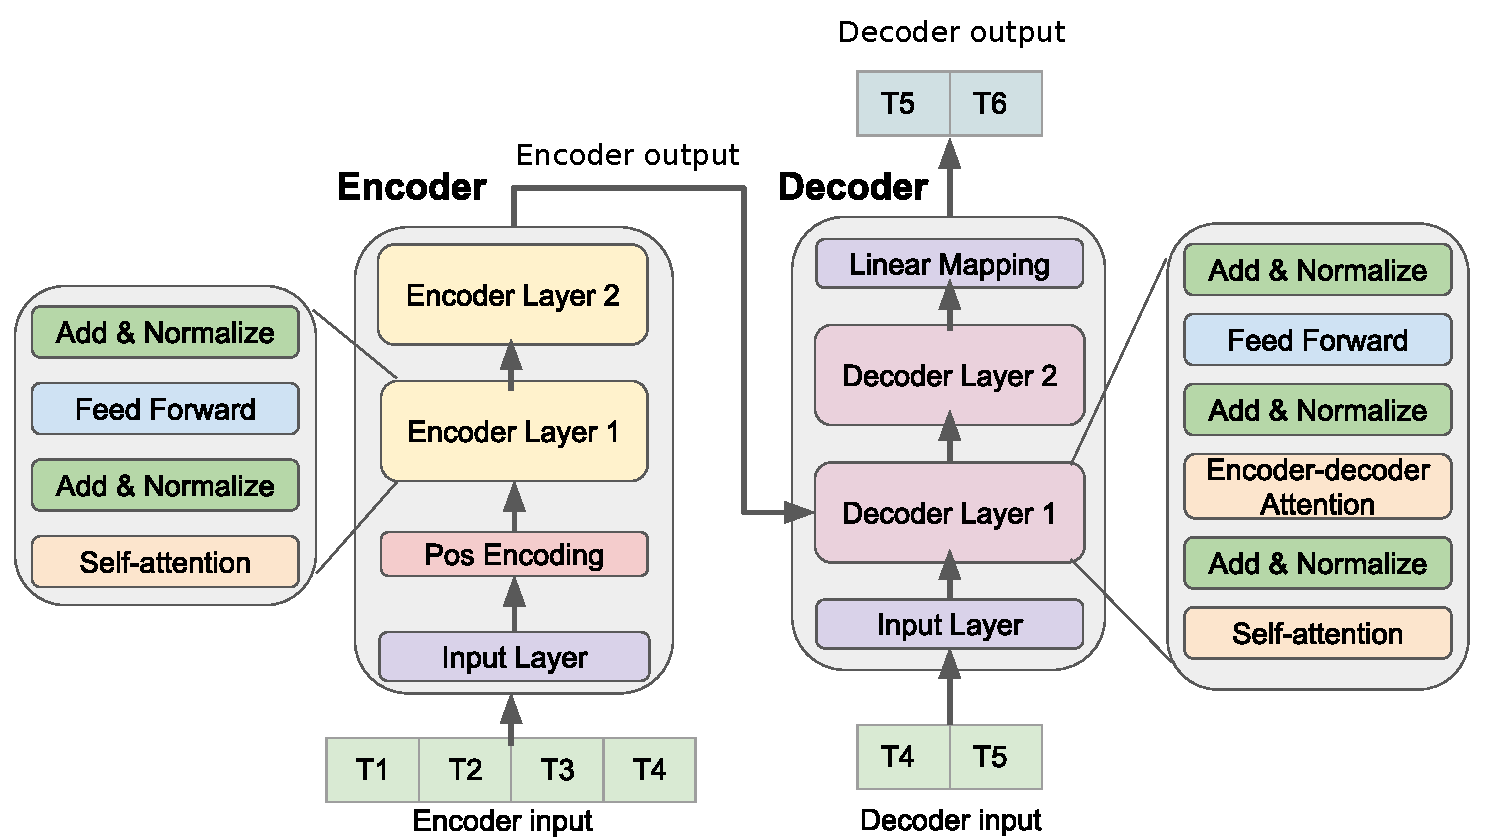
\includegraphics[width=\textwidth]{transformer_architecture.pdf}
    \caption{基于Transformer的预测模型架构}
  \end{figure*}
  
  \section{相关工作}
  一些研究使用互联网数据,如Google Trends、Twitter和Wikipedia来预测流感样似症比例。
  Google流感趋势(GFT)采用线性模型,利用预定义术语的Google搜索量来估计当前的流感样似症比例(“即时预测”)。
  尽管最初被认为是巨大的成功,但GFT在随后的几年中高估了峰值流感样似症数量。
  
  其他研究将GFT与新的建模技术和额外信号结合起来。
  Lazer等人提出了一种基于自回归(AR)的方法来扩展GFT。
  Santillana等人通过开发一种自动选择查询和更新流感样似症预测模型的模型,改进了GFT。
  Araz等人使用GFT数据和额外信号构建线性回归模型。
  Yang等人开发了一种基于自回归的模型,利用Google搜索数据(“ARGO”)来估计流感流行病。
  ARGO优于先前基于Google搜索的模型。
  最近,基于ARGO开发了一种新的集成模型(“ARGONet”)。
  这种新方法利用空间信息改进了模型,并实现了流感样似症预测的最新成果。
  
  深度学习技术也被用于流感样似症预测。
  Liu等人使用Google Trends、气候、空气污染和病毒学监测数据训练了基于LSTM的模型来预测流感流行程度。
  Venna等人开发了一个基于LSTM的多阶段模型,结合气候和时空调整因素进行流感预测。
  注意力机制也被应用于流感样似症预测。
  Zhu等人开发了多通道LSTM神经网络,可以从不同类型的输入中进行学习。
  他们的模型使用注意力层将模型输出与输入序列关联起来,进一步提高了预测的准确性。
  Kondo等人将序列到序列(“Seq2Seq”)模型与类似的注意力机制相结合,用于预测流感流行程度,并表明他们的方法优于ARIMA和基于LSTM的模型。
    
  \section{背景}
  \subsection{流感和流感样似症(ILI)}
  流感是一种由流感病毒感染引起的常见传染病。每年流感影响多达3500万人,给健康和经济带来巨大负担。在美国,疾病控制与预防中心(CDC)在一个广阔的地理区域内协调一个报告网络。网络中的参与健康提供者报告显示流感样似症(ILI)症状的患者统计数据。ILI症状通常定义为“发烧和咳嗽和/或喉咙痛”。ILI比例被计算为患有ILI症状的患者数量与当周总门诊人数的比值。CDC发布了美国和除佛罗里达州外的所有个别州的ILI比例。此外,州级的ILI比例还经过了对州人口的归一化处理。
  
  \subsection{状态空间模型}
  状态空间模型(State Space Models,SSM)广泛应用于动态系统。动态系统的演变受到不可观测的状态变量的控制。系统展现出由状态变量决定的可观测变量。SSM已应用于生物学和金融等复杂系统的研究中。
  
  状态空间模型同时建模状态变量和可观测变量。
  例如,广义线性状态空间模型可以用以下方程表示:
\begin{align}
x_t &= Z_t\alpha_t + \epsilon_t  \label{obs:eqn} \\
\alpha_{t+1} &= T_t\alpha_t + R_t\eta_t,  t = 1, ..., n, \label{state:eqn}
\end{align}
其中,$x_t$和$\alpha_t$分别是时间索引的观测向量和状态向量。
方程~\ref{obs:eqn}称为观测方程,它类似于回归方程。
它建模了可观测变量$x_t$与潜在状态变量$\alpha_t$之间的关系。
方程~\ref{state:eqn}是状态方程,具有自回归性质。
它控制了状态变量随时间的演变。
$\epsilon_t$和$\eta_t$是创新项,通常被建模为高斯过程。
在这一节中,我们简要提及了一些在ILI预测中常用的SSM模型。

\paragraph*{隔室模型}
隔室模型是SSM的一种特定形式,广泛应用于研究传染病。在隔室模型中,将人群分为不同的组(“隔室”)。每个组通过一个时间相关的状态变量来建模。一个著名的隔室模型是“易感-感染-康复”(Suscepted-Infected-Recovered,SIR)模型,该模型通过以下常微分方程来描述系统的演变:
\begin{align*}
\frac{dS}{dt} &= -\frac{\beta IS}{N}\\
\frac{dI}{dt} &= \frac{\beta IS}{N} - \gamma I\\
\frac{dR}{dt} &= -\gamma I
\end{align*}
在这个模型中,ILI时间序列是系统的可观测变量:$\mathrm{ILI}(t) = I(t) / (I(t) + S(t) + R(t))$。
尽管最初是为了建模传染病而开发的,隔室模型已被应用于生态学和经济学等其他学科。
虽然隔室模型很有用,但它们需要对微分方程的参数具有先验知识,并且缺乏在新观测数据下更新参数的灵活性。
    \paragraph*{ARIMA}
Box-Jenkins ARIMA(自自回归差分移动平均)是另一种常用的建模动态系统的方法。ARIMA模型对观测变量$x_t$进行建模,假设$x_t$可以分解为趋势、季节性和随机的成分。Box和Jenkins的想法是对时间序列$x_t$进行差分操作,以消除趋势和季节性。得到的序列被视为平稳时间序列数据,并使用其滞后时间序列值的组合(“AR”)和滞后预测误差的移动平均值(“MA”)进行建模。ARIMA模型通常由一个元组$(p, d, q)$来指定,其中$p$和$q$定义了AR和MA的阶数,$d$指定了差分操作的阶数。

ARIMA可以用SSM形式来表示,常见的SSM技术如滤波和平滑也可以应用于ARIMA。然而,ARIMA是一种“黑盒”方法,模型完全依赖于观测数据,没有对潜在系统状态的分析。

\paragraph*{时间延迟嵌入}
对于标量时间序列数据$x_t$,其时间延迟嵌入(TDE)是通过将每个标量值$x_t$嵌入到$d$维的时间延迟空间中形成的:
\begin{equation*}
\mathrm{TDE_{d, \tau}}(x_t) = (x_t, x_{t-\tau}, ..., x_{t-(d-1)\tau}) % TODO(neowu) check if whether this the right definition?
\end{equation*}
对于任何非线性动力系统而言,延迟嵌入定理(Takens定理)表明存在某个$(d, \tau)$-时间延迟嵌入,可以通过观测变量的延迟坐标近似恢复出原始状态变量(即“相空间”)的演化。在流感样似症预测的情况下,Takens定理表明通过对ILI比例(即“观测变量”)构造的$\mathrm{TDE_{d, \tau}}$,可以近似描述由生物学和物理机制控制的潜在动力系统。

Sugihara和May在开创性工作中首次探索了TDE在时间序列预测中的应用。他们展示了TDE可以通过对系统动力学的定性评估,无需了解底层机制,实现短期预测。他们开发了基于TDE的模型来预测水痘和麻疹的发病率,并将其与基于AR的方法进行比较。他们的分析表明,对于水痘病例的预测,TDE模型与AR模型表现相当,而对于麻疹病例的预测,TDE模型优于AR模型。

在状态空间模型(SSM)框架中,时间延迟嵌入是一种强大的工具,可以通过学习底层动力系统的几何和拓扑信息,将状态变量和观测数据联系起来,而无需理解系统的状态变量和相空间。尽管TDE具有令人惊叹的特性,但据我们所知,TDE在机器学习模型中尚未得到广泛研究。

\subsection{序列模型}
许多现实世界的机器学习任务涉及不同类型的序列数据,包括自然语言文本、音频和视频、DNA序列和时间序列数据。序列模型专门用于建模这种数据。在本节中,我们简要回顾几种常见的序列模型。

\paragraph*{循环神经网络}
与传统的前馈网络不同,循环神经网络(Recurrent Neural Networks,RNN)具有循环性质 - 它对每个输入$x_t$执行相同的函数,并且输出$y_t$依赖于输入$x_t$和前一个状态$h_{t-1}$。

\begin{figure}
\centering
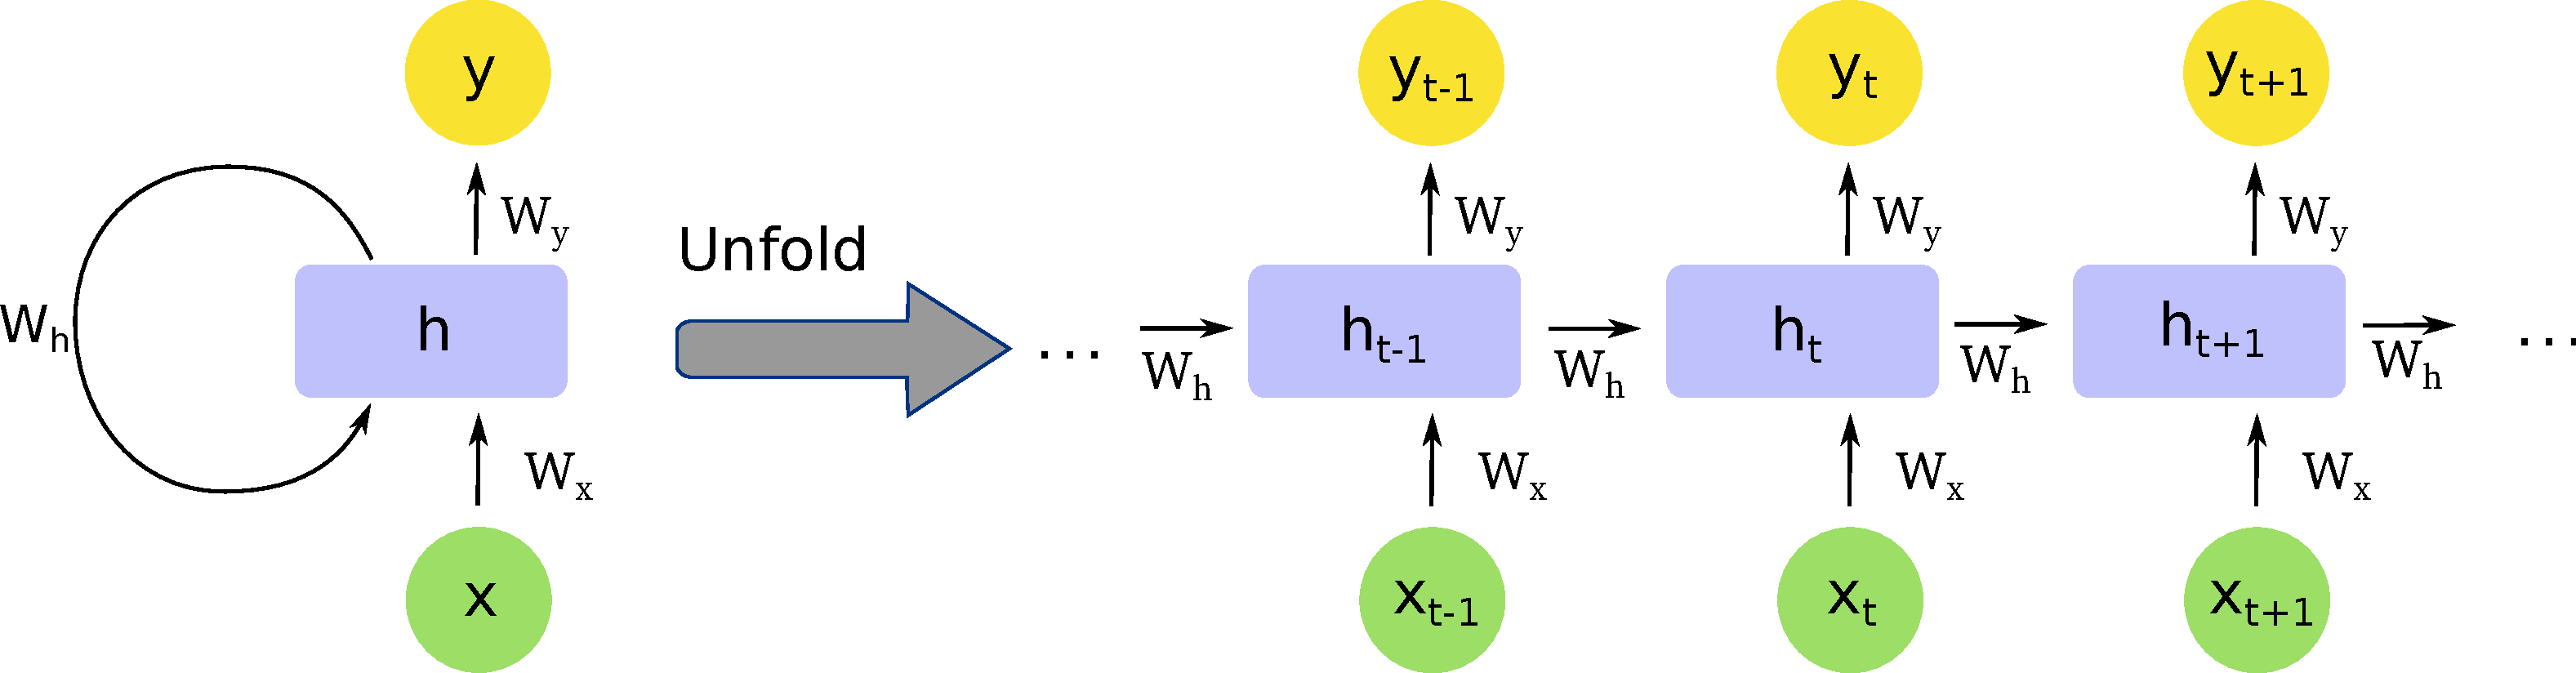
\includegraphics[width=16cm,height=10cm,keepaspectratio]{rnn.pdf}
\caption{循环神经网络的折叠和展开表示}
\label{fig:rnn}
\end{figure}

如图~\ref{fig:rnn}所示,简单的循环神经网络(Simple RNN)可以表示为:
\begin{align*}
h_t &= \sigma(W_x x_t + W_h h_{t-1} + b_h) \\
y_t &= \sigma(W_y h_t + b_y)
\end{align*}
其中,$x_t$是输入向量,$h_t$是隐藏状态向量,$y_t$是输出向量。$W$和$b$是学习参数,$\sigma$是激活函数。

\paragraph*{长短期记忆网络(LSTM)}
虽然循环神经网络具有处理序列数据的内部记忆,但在处理长序列时会出现梯度消失和爆炸的问题。为了解决这个限制,专门开发了长短期记忆(Long Short-Term Memory,LSTM)网络。LSTM使用三个门,包括输入门、遗忘门和输出门,来调节细胞之间的信息流动,防止梯度消失和爆炸。

\begin{figure}
\centering
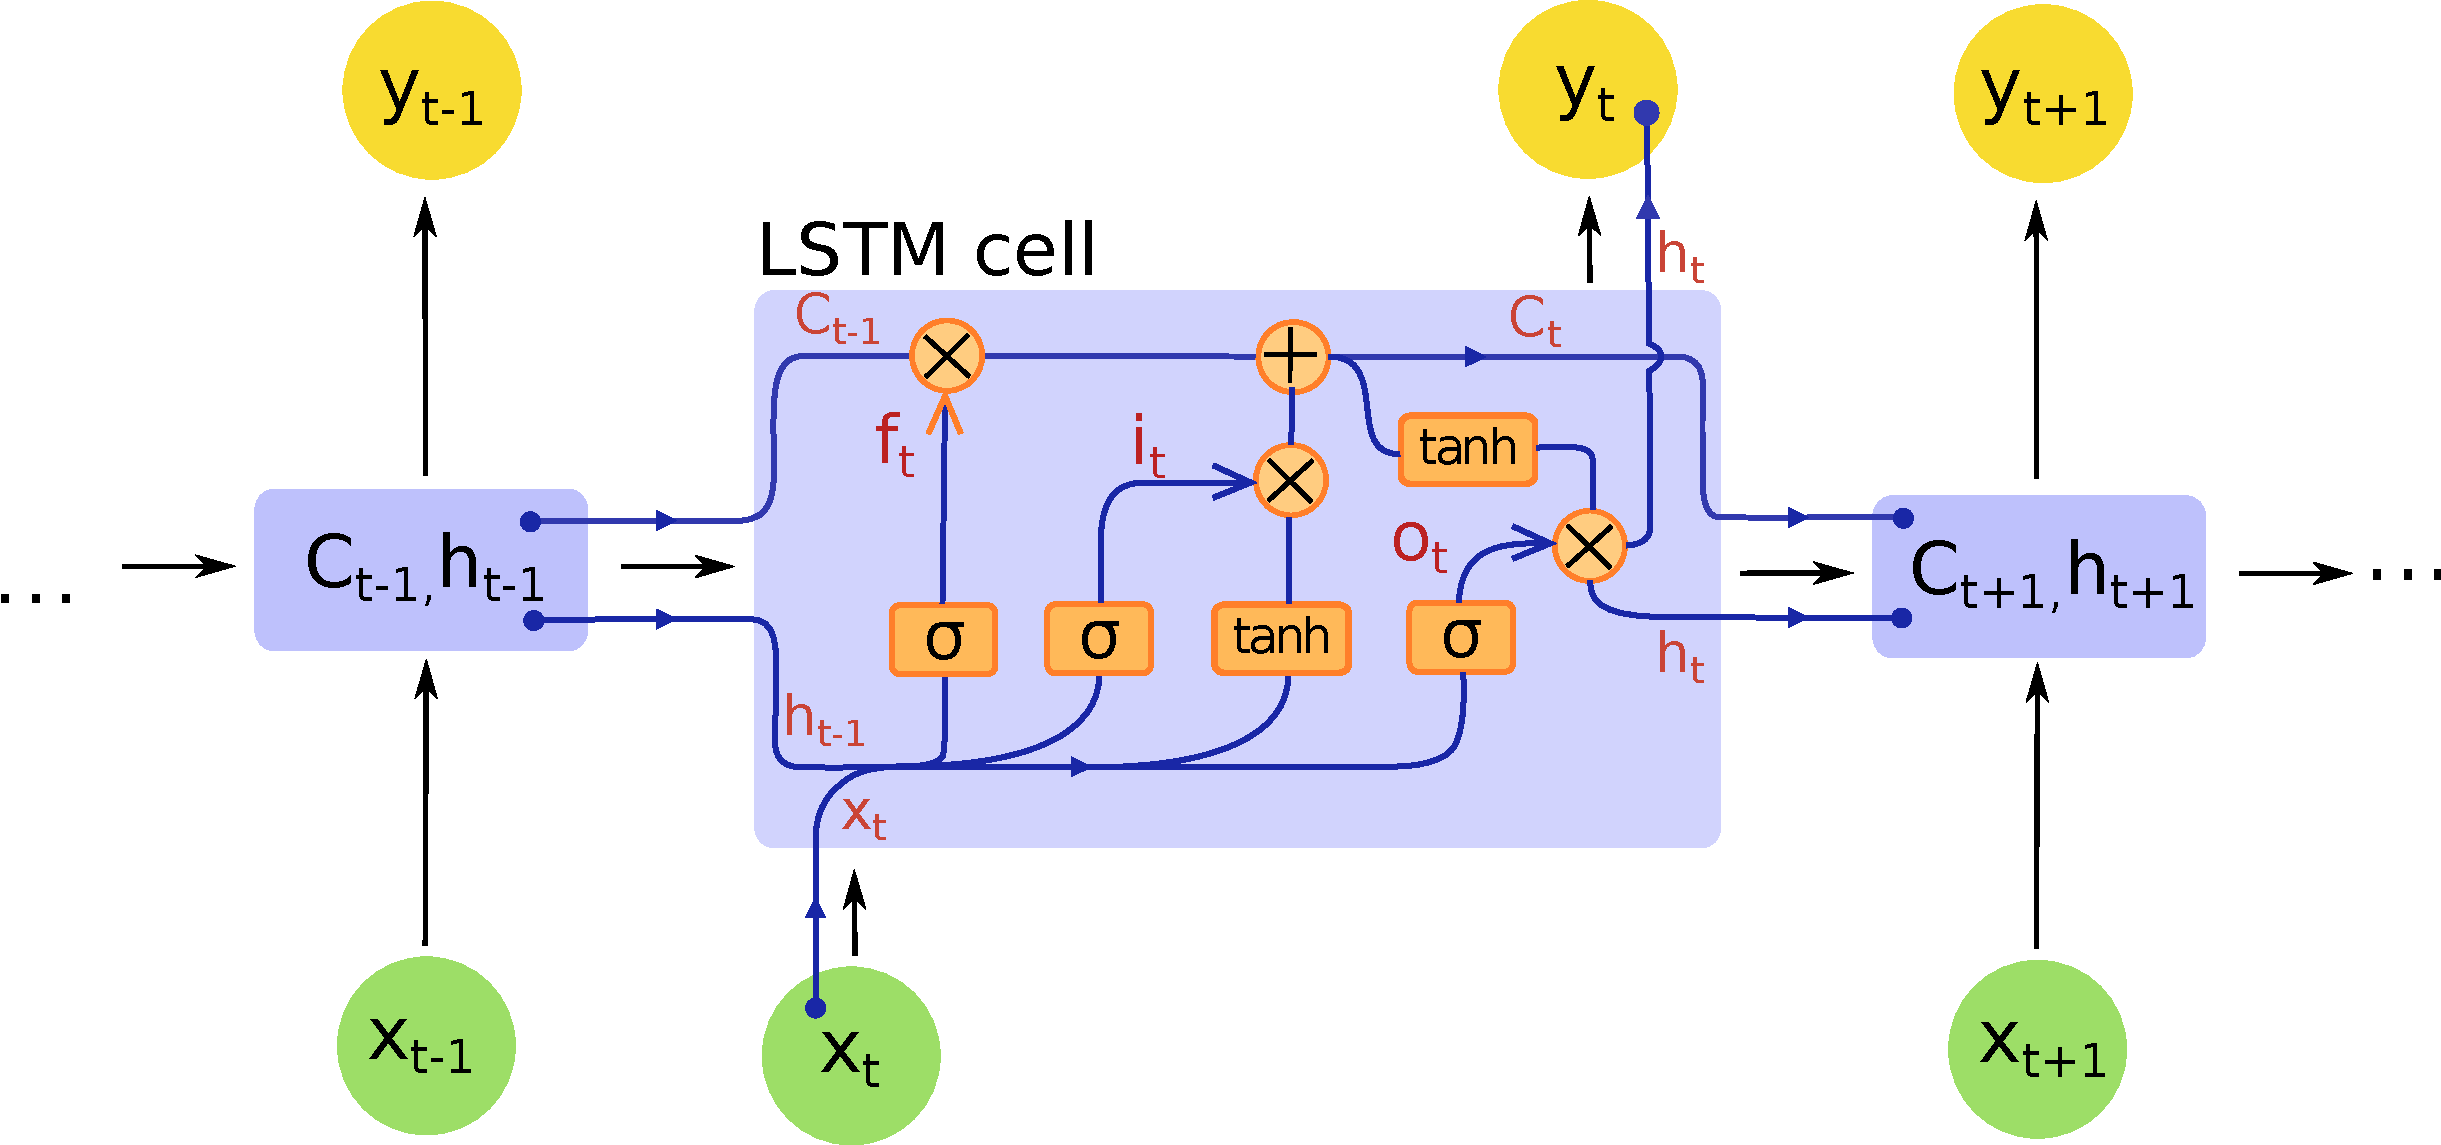
\includegraphics[width=16cm,height=10cm,keepaspectratio]{lstm.pdf}
\caption{长短期记忆网络和LSTM单元}
\end{figure}
\begin{align*}
f_t &= \sigma(W_f [h_{t-1}, x_t] + b_f) \\
i_t &= \sigma(W_i [h_{t-1}, x_t] + b_i) \\
\tilde{C_t} &= \tanh(W_C [h_{t-1}, x_t] + b_C) \\
C_t &= f_t * C_{t-1} + i_t * \tilde{C_t} \\
y_t &= \sigma(W_y [h_{t-1}, x_t] + b_y) \\
h_t &= y_t * \tanh(C_t)
\end{align*}
\paragraph*{序列到序列模型(Seq2Seq)}
序列到序列(Sequence-to-Sequence,Seq2Seq)架构是为了处理输入和输出都是序列的机器学习任务而开发的。Seq2Seq模型由三个组件组成,包括编码器(Encoder)、中间向量(Intermediate Vector)和解码器(Decoder)。编码器是一堆LSTM或其他循环单元。每个单元接收输入序列中的一个元素。编码器的最终隐藏状态被称为编码器向量或上下文向量,它编码了输入数据的所有信息。解码器也由一堆循环单元组成,并以编码器向量作为其第一个隐藏状态。每个循环单元计算自己的隐藏状态并产生一个输出元素。图~\ref{fig:seq2seq}展示了Seq2Seq架构。

Seq2Seq在语言翻译任务中得到了广泛应用。然而,它在处理长句子时性能下降,因为它无法充分将长序列编码到中间向量中(即使使用LSTM单元)。因此,在编码器向量中往往会丢失长期依赖关系。

\begin{figure}
\centering
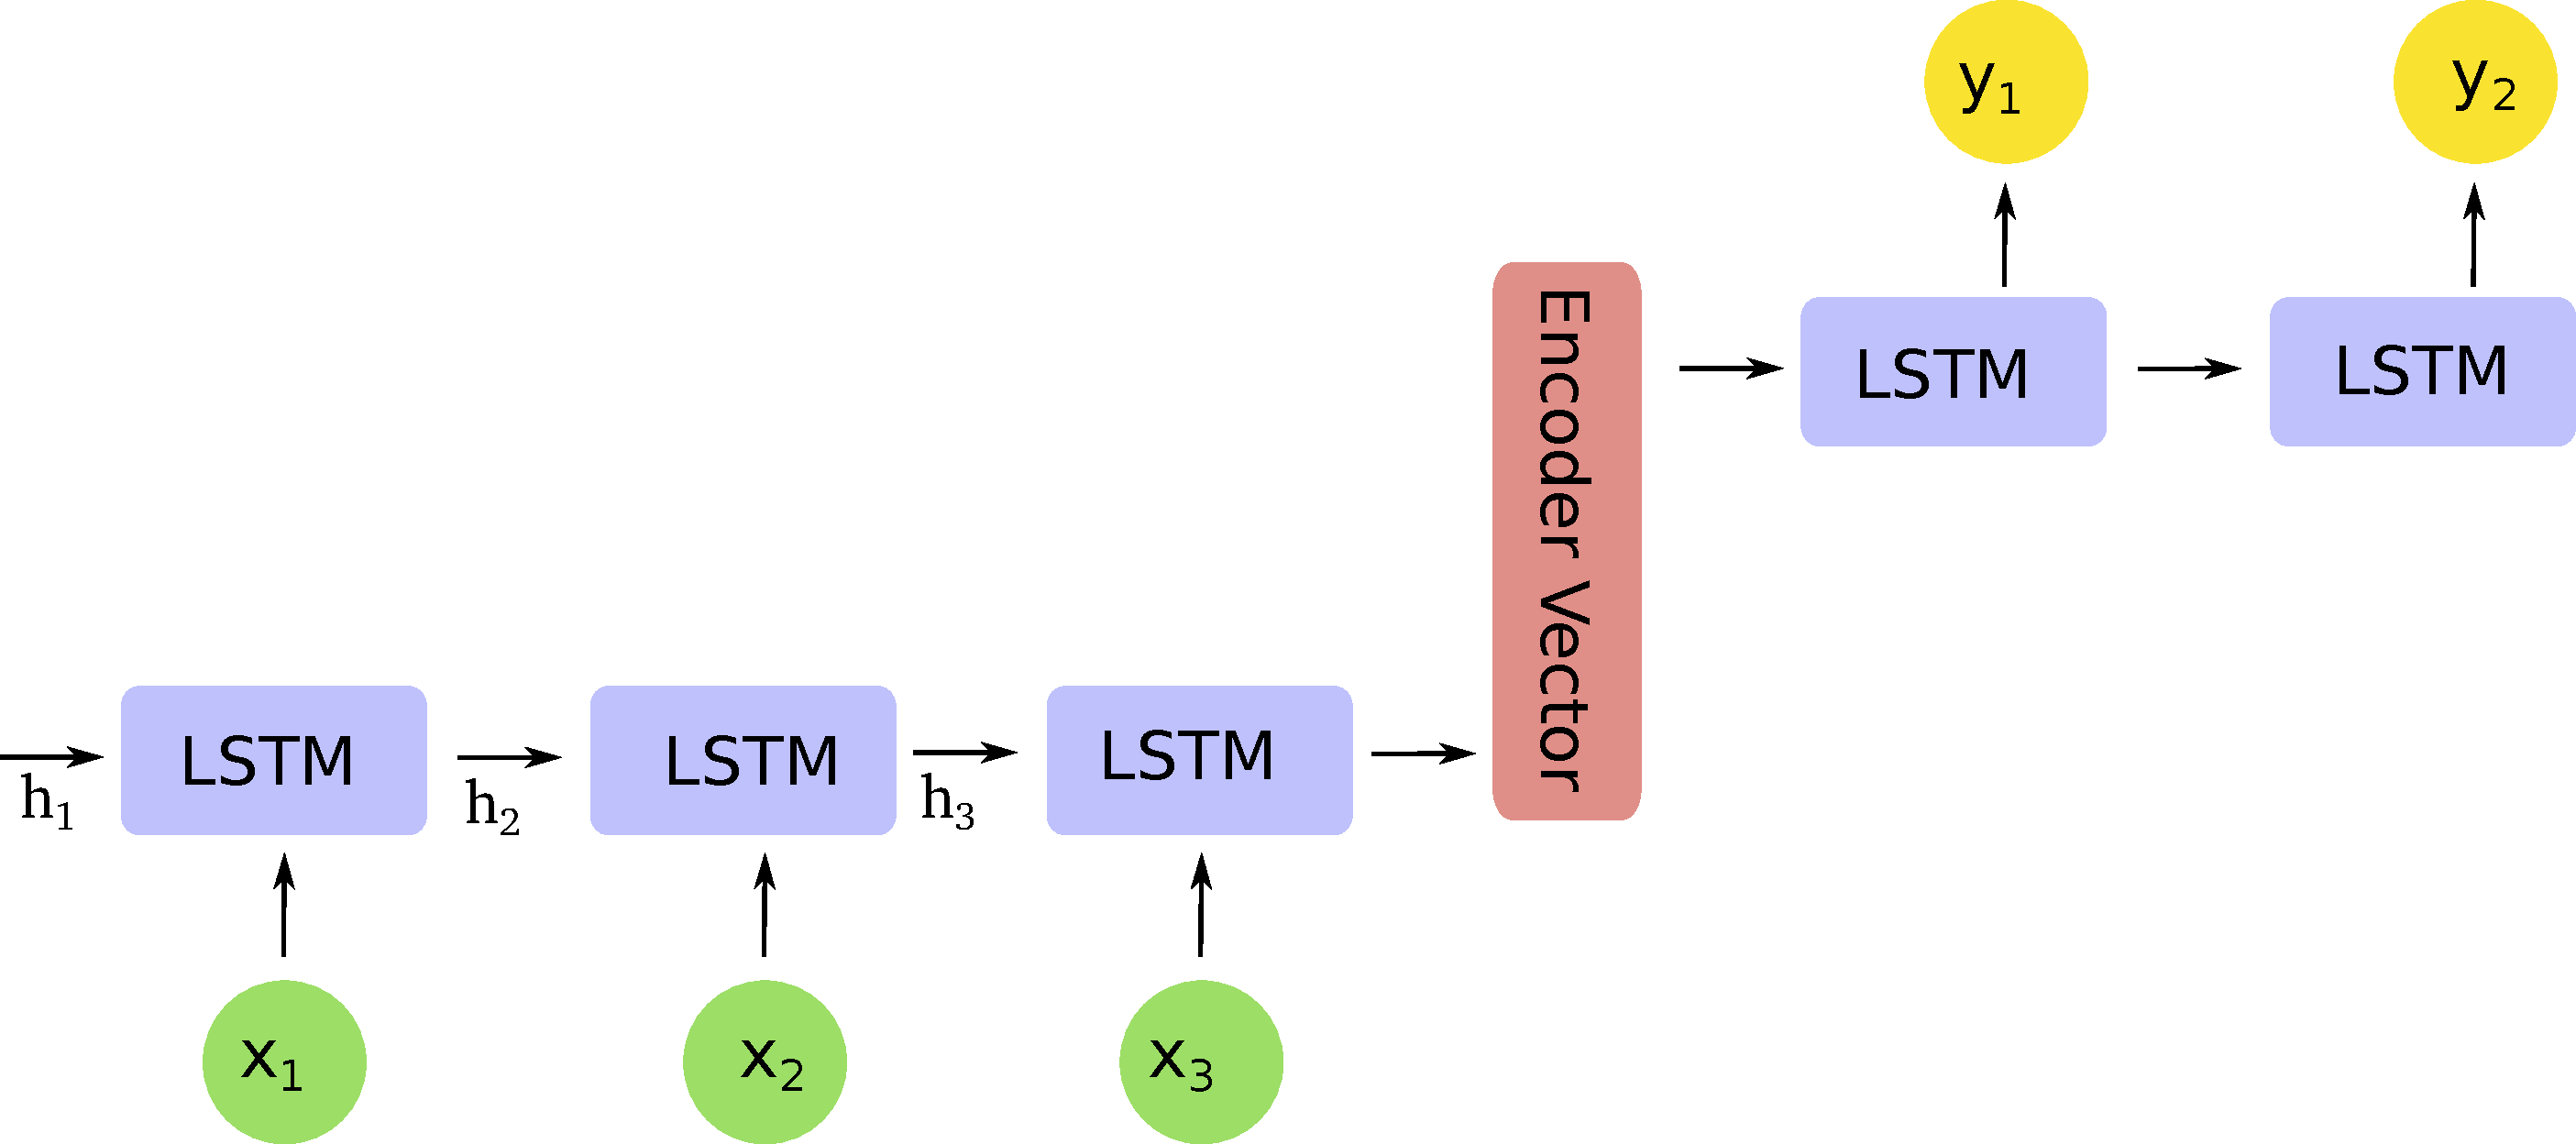
\includegraphics[width=12cm,height=6cm,keepaspectratio]{seq2seq.pdf}
\caption{序列到序列模型架构}
\label{fig:seq2seq}
\end{figure}
    
    
    \section{模型}
    \subsection{问题描述}
    我们将ILI预测问题建模为一个监督机器学习任务。给定包含$N$个周数据点的时间序列${x_{t-N+1}, ..., x_{t-1}, x_t}$,对于$M$步预测,监督机器学习模型的输入$X$为${x_{t-N+1}, ..., x_{t-M}}$,输出$Y$为${x_{t-M+1}, x_{t-M+2}, ..., x_t}$。每个数据点$x_t$可以是一个标量或包含多个特征的向量。
 
    \subsection{数据}
我们利用了来自CDC的2010年至2018年的国家和州级历史ILI数据。

为了生成带标签的数据集,我们采用了固定长度的滑动时间窗口方法(图~\ref{fig:sliding-window}),构建用于模型训练和评估的${X, Y}$对。在应用滑动窗口之前,我们对所有数据进行最大最小值缩放,使用训练数据集的最大和最小值。然后在缩放后的训练集上运行滑动窗口,获得具有特征和标签的训练样本,其中特征是前N个观测值,标签是后M个观测值。测试样本也以相同的方式构建,用于模型评估。训练和测试集的划分比例为2:1。来自不同州的训练数据被连接起来形成全局模型的训练集。

\begin{figure}
\centering
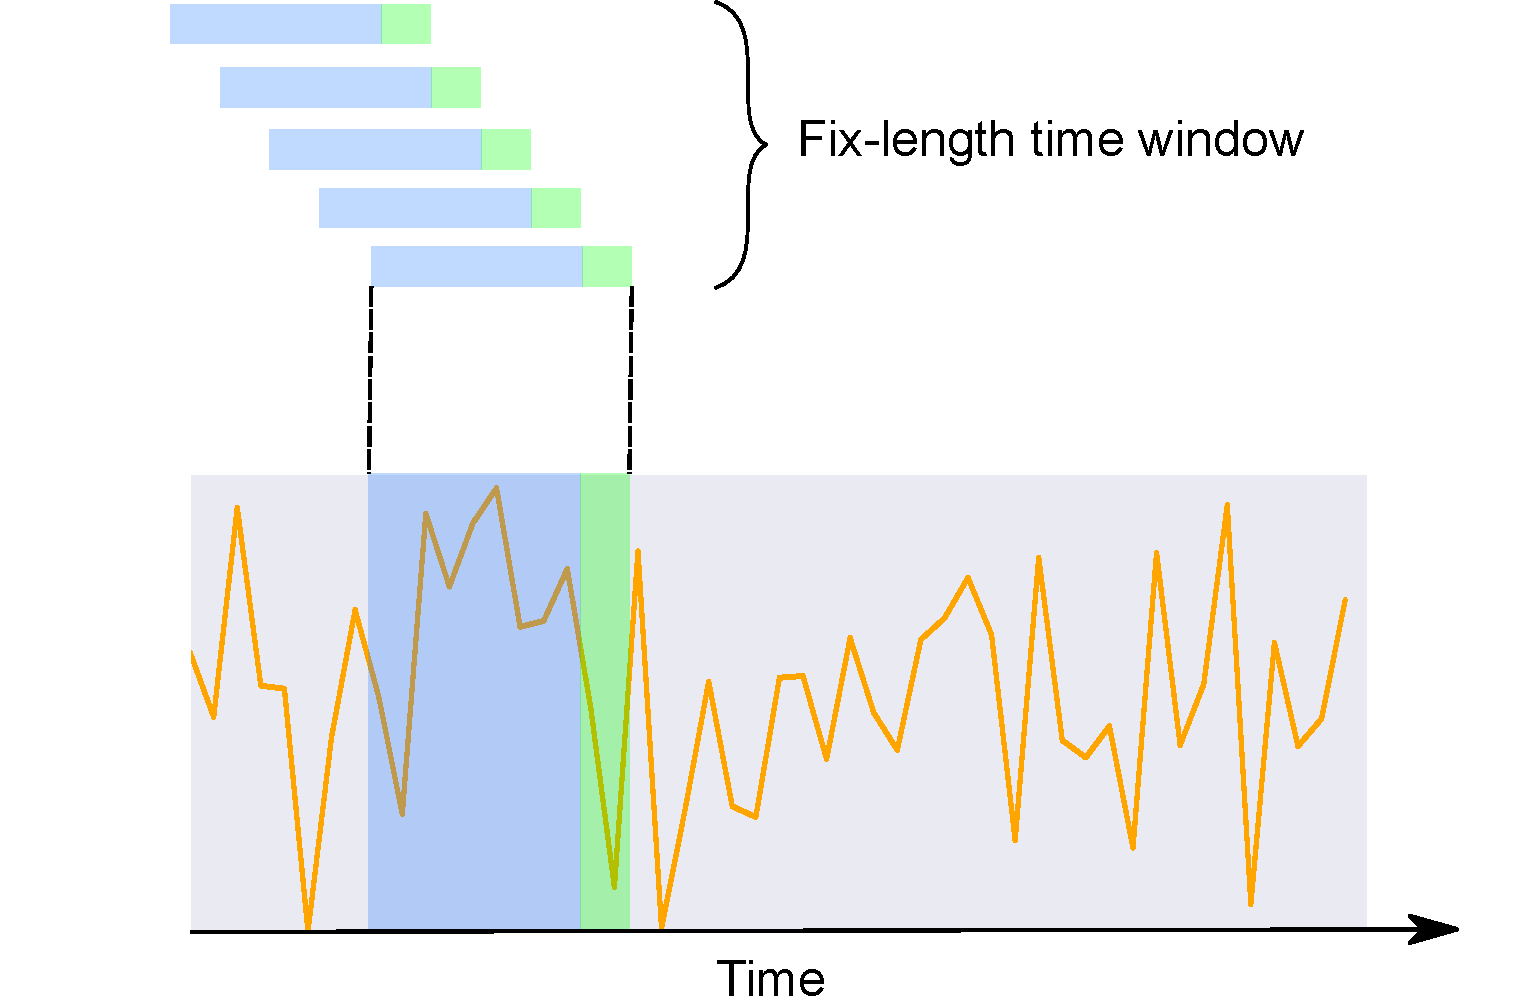
\includegraphics[width=16cm,height=10cm,keepaspectratio]{sliding_window.pdf}
\caption{使用滑动时间窗口构建训练样本和测试样本}
\label{fig:sliding-window}
\end{figure}
    
    \subsection{Transformer模型}
    \subsubsection{模型架构}
    我们基于原始的Transformer架构构建了基于Transformer的ILI预测模型,包括编码器和解码器层。
    
    \paragraph*{编码器}
    编码器由输入层、位置编码层和四个相同的编码器层组成。
    输入层通过一个全连接网络将输入的时间序列数据映射为一个维度为$d_{\text{model}}$的向量。这一步对于模型使用多头注意力机制至关重要。
    使用正弦和余弦函数的位置编码对时间序列数据中的顺序信息进行编码,通过将输入向量与位置编码向量进行逐元素相加来实现。
    得到的向量被馈送到四个编码器层。每个编码器层包括两个子层:自注意力子层和全连接前馈子层。每个子层之后都有一个归一化层。
    编码器产生一个$d_{\text{model}}$维的向量,用于馈送给解码器。

\paragraph*{解码器}
我们采用了与原始Transformer架构相似的解码器设计。
解码器由输入层、四个相同的解码器层和一个输出层组成。
解码器的输入从编码器输入的最后一个数据点开始。
输入层将解码器输入映射为一个维度为$d_{\text{model}}$的向量。
除了每个编码器层中的两个子层外,解码器还插入第三个子层,对编码器输出应用自注意力机制。
最后,有一个输出层将最后一个解码器层的输出映射到目标时间序列。
在解码器中,我们采用前瞻遮挡和解码器输入与目标输出之间的一位偏移,以确保对时间序列数据点的预测仅依赖于先前的数据点。

\subsubsection{训练}
\paragraph*{训练数据和批处理}
在典型的训练设置中,我们训练模型从过去10个周的数据预测未来4周的ILI比例。
也就是说,给定编码器输入$(x_1, x_2, ..., x_{10})$和解码器输入$(x_{10}, ..., x_{13})$,解码器的目标是输出$(x_{11}, ..., x_{14})$。
我们使用前瞻遮挡来确保模型只会在目标数据之前的数据点上应用注意力。
也就是说,在预测目标$(x_{11}, x_{12})$时,遮挡确保注意力权重仅作用在$(x_{10}, x_{11})$上,以防止解码器从解码器输入中泄露关于$x_{12}$和$x_{13}$的信息。
训练时使用大小为64的小批量数据。
\paragraph*{优化器}
我们使用Adam优化器,其中$\beta_1 = 0.9$,$\beta_2 = 0.98$,$\epsilon = 10^{-9}$。
我们使用自定义的学习率和以下调度表进行训练:
\begin{align*}
lrate = &d_{\text{model}}^{0.5} * \min(\text{step\_num}^{0.5},\\
        &\text{step\_num} * \text{warmup\_steps}^{-1.5})
\end{align*}
其中$\text{warmup\_steps} = 5000$。

\paragraph*{正则化}
我们对编码器和解码器中的三种子层(自注意力子层、前馈子层和归一化子层)都应用了dropout技术。
每个子层的dropout率为0.2。

\subsubsection{评估}
在评估中,我们使用固定长度的滑动窗口构建了带有标签的测试数据。
经过训练的Transformer模型进行一步预测。
我们计算实际数据${y_i}$和预测值${\hat{y_i}}$之间的皮尔逊相关系数和均方根误差(RMSE)进行评估。
\subsection{ARIMA、LSTM和Seq2Seq模型}
本节介绍了我们开发的其他模型,用于对比Transformer-based模型的性能。

\paragraph*{ARIMA}
我们使用ARIMA模型作为基准模型。ARIMA模型将时变的ILI比例视为一个遵循固定动态的单变量时间序列。每周的ILI比例取决于前$p$周的观测值和前$q$周的估计误差。我们使用赤池信息准则(AIC)和贝叶斯信息准则(BIC)来选择ARIMA模型的阶数,以在模型复杂性和泛化性之间取得平衡。我们选择了$\mathrm{ARIMA}(3,0,3)$的阶数,并添加了一个常数趋势,以保持模型的简洁性。该模型基于状态空间建模框架进行训练,使用数据集的前三分之二进行训练。然后,使用拟合的参数对完整的时间序列进行滤波,进行四步的预测。

\paragraph*{LSTM}
LSTM模型由两个LSTM层的堆叠和一个最后的全连接层组成,直接预测多步的ILI比例。LSTM层通过循环网络从输入中编码顺序信息。全连接层接收来自第二个LSTM层的最终输出,并输出一个大小为4的向量,与预测的步数相对应。两个LSTM层分别具有32个和16个单元。为了正则化,我们在LSTM层中应用了0.2的丢弃率。训练时使用Huber损失、Adam优化器和学习率为0.02。

\paragraph*{Seq2Seq}
Seq2Seq模型采用了一种与Transformer模型类似的编码器-解码器架构,不过它并没有使用自注意力机制。它的编码器和解码器都由两层LSTM构成。编码器的作用是将输入的序列转化为一个上下文向量,然后解码器利用这个上下文向量以及前一个输出逐步生成目标序列。在训练这个Seq2Seq模型的过程中,我们采用了Huber损失、Adam优化器和0.02的学习率。

Seq2Seq模型的主要用途是作为基准模型,用来与基于Transformer的模型进行对比和性能评估。

\paragraph*{Seq2Seq}
我们测试的Seq2Seq模型也采用了编码器-解码器架构,编码器部分由一个全连接的稠密层
和一个GRU(门控循环单元)层组成,其主要任务是从输入的序列中提取和学习特征,最
终返回一组编码的输出和最后一个隐藏状态。解码器的结构设计与编码器部分基本相同
。在这个模型中,稠密层包含16个单元,而GRU层则包含32个单元。值得一提的是,这
个Seq2Seq模型还巧妙地融入了注意力机制。具体来说,解码器在每一步的解码过程
,都会利用Bahdanau注意力机制处理编码器的输出序列,以便更好地进行下一步的预
测。解码器还使用了一种名为“Teacher forcing”的技术,这有助于模型更快地收敛
,同时解决了不稳定性问题。这种技术的基本思路是,在训练过程中,我们会将当前时
间步的真实ILI比例作为下一个时间步的输入,而不是使用解码器单元计算出的输出。
此外,为了防止过拟合,所有的循环层中都采用了0.2的丢弃率。在训练这个模型的过
程中,我们使用了Huber损失函数、Adam优化器和0.02的学习率。
\section{实验}
\subsection{仅使用ILI数据进行一步预测}
\begin{figure*}
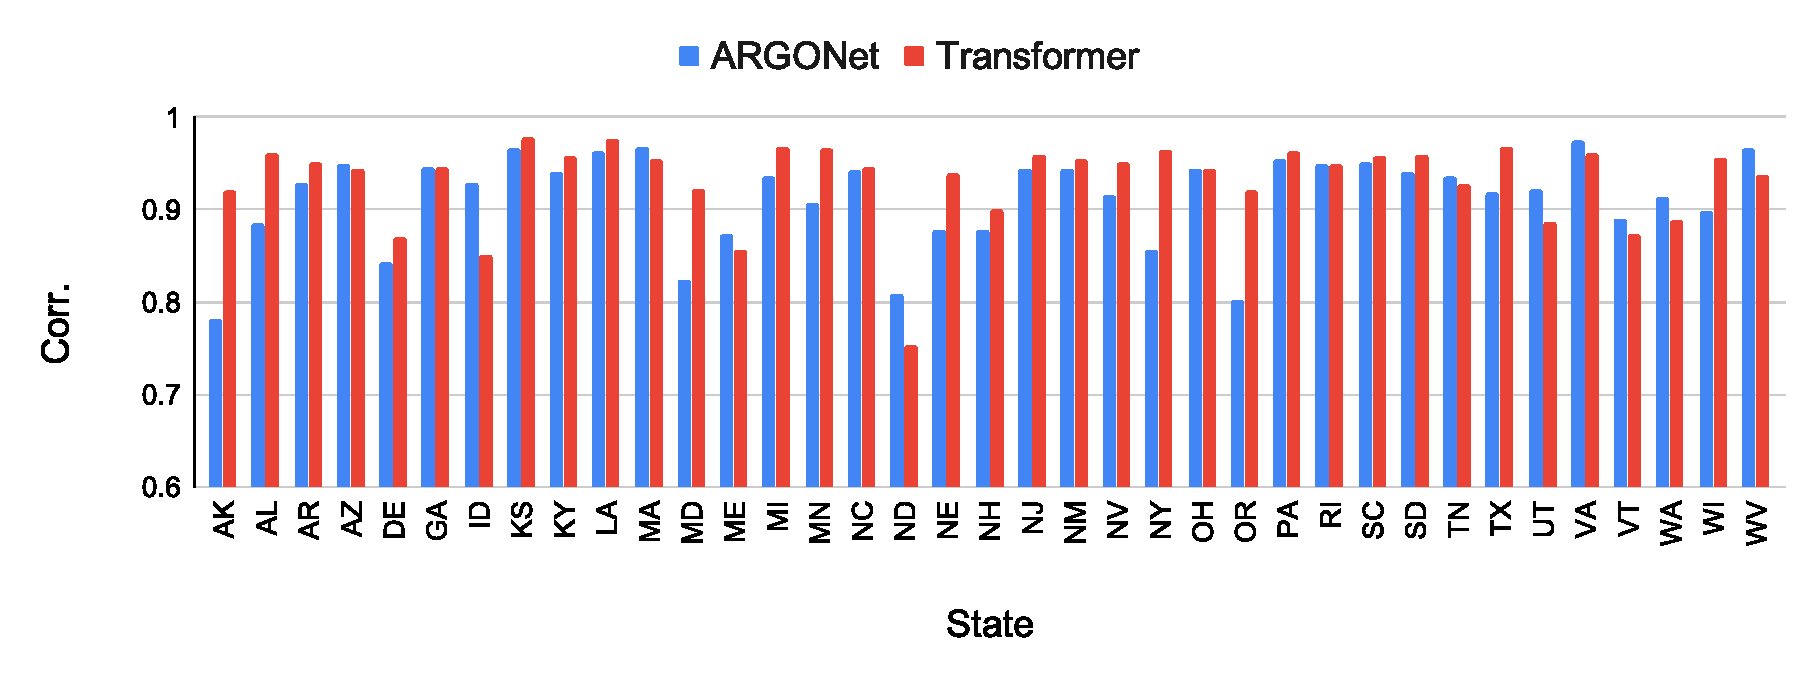
\includegraphics[width=\textwidth]{argo_transformer_corr.pdf}
\caption{ARGONet和Transformer模型的皮尔逊相关系数}
\label{fig:argo_transformer_corr}
\end{figure*}
\begin{figure*}
    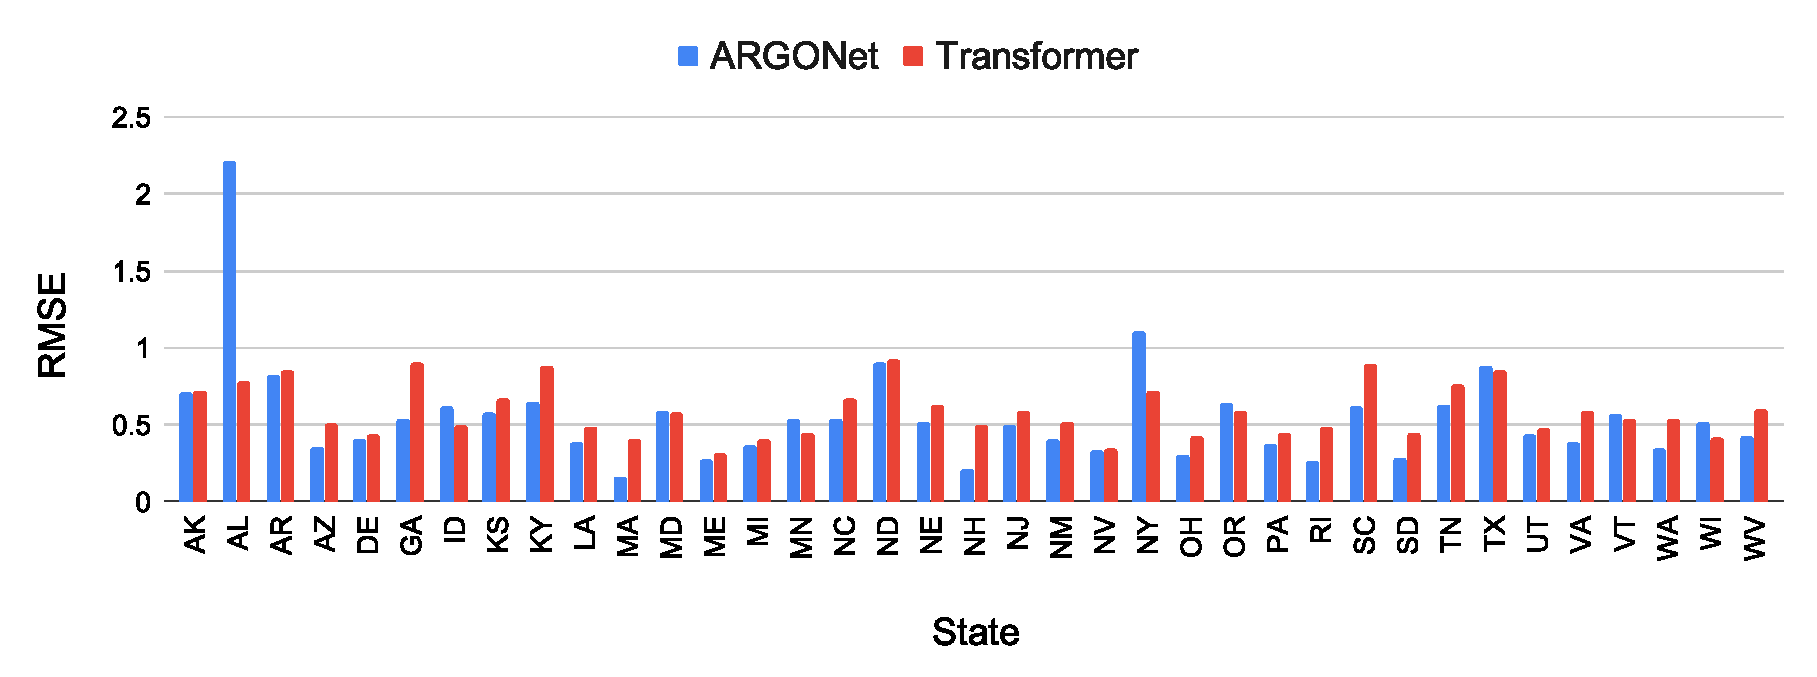
\includegraphics[width=\textwidth]{argo_transformer_rmse.pdf}
    \caption{ARGONet和Transformer模型的均方根误差(RMSE)}
    \label{fig:argo_transformer_rmse}
    \end{figure*}
    
    在我们的第一个实验中,我们测试了我们基于Transformer的模型是否能够从历史数据中预测一周后的ILI比例。为了评估模型,训练好的全局模型使用测试数据集进行一步预测。计算了每个州的皮尔逊相关系数和均方根误差(RMSE)。
    
    我们将Transformer模型的性能与ARIMA、LSTM和带有注意力机制的Seq2Seq模型进行
    了比较。表~\ref{table:exp_compare}总结了每种方法的相关系数和RMSE,以及相
    对于ARIMA方法的性能提升。比较表明,深度学习模型在相关系数和RMSE方面整体优于
    ARIMA。在这三种深度学习方法中,相关系数非常接近,Transformer模型略高于
    LSTM和带有注意力机制的Seq2Seq模型。在RMSE方面,Transformer模型的
    性能优于LSTM和带有注意力机制的Seq2Seq模型,相对的RMSE减小分别为27%和8.4%
    。这个分析表明,注意力机制对预测性能起到了贡献,因为带有注意力机制的Seq2Seq
    和Transformer模型优于纯LSTM模型。此外,与带有注意力机制的Seq2Seq模型相
    比,Transformer模型显示出更好的预测性能,这表明Transformer的自注意机
    制能够更好地捕捉数据中的复杂动态模式。值得注意的是,Transformer在美国的
    ILI预测中显示出最佳的指标(皮尔逊相关系数=0.984,RMSE=0.3318)。由
    于单个模型使用来自所有州的数据进行训练,这表明该模型确实能够推广各个州
    的模式,用于国家级的预测。
    
    \begin{table}[h!]
        \centering
           \caption{模型性能总结及相对于基准模型的变化}
           \label{table:exp_compare}
           \begin{tabular}{| c || c | c ||}
           \hline
           模型 & 皮尔逊相关系数 & RMSE \\ [0.5ex]
           \hline\hline
           ARIMA &
             \begin{tabular}{@{}c@{}}0.769 \\ \small{(+0 \%)} \end{tabular} &
             \begin{tabular}{@{}c@{}} 1.020 \\ \small{(-0 \%)} \end{tabular}\\
             \hline
           LSTM &
             \begin{tabular}{@{}c@{}}0.924 \\ \small{(+19.9 \%)} \end{tabular} &
             \begin{tabular}{@{}c@{}} 0.807 \\ \small{(-20.9 \%)} \end{tabular}\\
             \hline
           Seq2Seq+注意力机制 &
             \begin{tabular}{@{}c@{}}0.920 \\ \small{(+19.5 \%)} \end{tabular} &
             \begin{tabular}{@{}c@{}} 0.642 \\ \small{(-37.1 \%)} \end{tabular}\\
             \hline
           Transformer &
             \begin{tabular}{@{}c@{}}0.928 \\ \small{(+20.7 \%)} \end{tabular} &
             \begin{tabular}{@{}c@{}} 0.588 \\ \small{(-42.4 \%)} \end{tabular} \\
             \hline
           \end{tabular}
        \end{table}
        \subsection{使用特征向量的逐步预测}
        接下来,我们测试了基于Transformer的模型是否能够从多个特征(即多变量时间序列数据)中学习进行ILI预测。
        在美国,流感季节通常从10月初开始,并在1月和2月之间达到高峰。
        我们假设周数是模型的一个信息量丰富的信号。
        因此,我们将“周数”作为一个与时间相关的特征引入模型中。
        此外,我们还在模型中包括时间序列的一阶和二阶差分作为两个显式的数值特征。

        我们的结果表明,包含这些特征可以提高模型的性能(平均皮尔逊相关系数:0.931,平均RMSE = 0.585)。
        然而,与仅使用ILI数据的Transformer模型相比,改进并不显著。
        这表明这些额外的特征可能对模型提供了较少的新信息。
        也就是说,如果基于Transformer的模型能够依赖自注意力机制从ILI时间序列中学习短期和长期依赖关系,那么引入的一阶和二阶差分特征很可能是多余的。
        
        我们将结果与ARGONet的ILI预测数据进行了比较,ARGONet是文献中的一种先进的ILI预测模型。
        图~\ref{fig:argo_transformer_corr}和图~\ref{fig:argo_transformer_rmse}显示了ARGONet和我们的Transformer模型的相关系数和RMSE值。
        总体而言,基于Transformer的模型与ARGONet的性能相当,平均相关系数略有改善(ARGONet: 0.912,Transformer: 0.931),平均RMSE值略有下降(ARGONet: 0.550,Transformer: 0.593)。
        
        \subsection{采用时间延迟嵌入法进行预测分析}

        在这一部分,我们针对基于Transformer的模型能否直接对动力系统的相空间进行建模进行了一番实验探究。我们采用了历史的ILI数据,以此构建出时间延迟嵌入(TDEs)。值得注意的是,当TDEs的维度足够多时,它在拓扑结构上就能等同于那些未知的动力系统相空间。
        
        换句话说,相对于我们观测到的标量变量ILI数据,TDEs所编码的内容包含了更丰富的几何和拓扑信息,这些信息是控制流感感染和传播过程的系统必需的。因此,如果我们采用TDEs,就能获取到比标量时间序列输入更丰富的信息。
        
        为了检验这个理论,我们从ILI数据中构建了从2到32维的时间延迟嵌入,并以此作为特征,进行基于Transformer的ILI预测。在表\ref{tde:dim}中,我们列出了在不同TDE维度$d$下的预测指标结果。在所有的实验中,我们均采用了$\tau=1$来构建TDEs。
        
        通过观察我们发现,改变TDE的维度并不会对皮尔逊相关系数产生显著影响。然而,在维度增加的过程中,RMSE值先是降低,后又趋于稳定,其中在维度为8时达到了最小值。这个结果与预测水痘和麻疹所使用的最优TDE维度相近,那时的最优维度分别为5和5-7。
        \begin{table}[h!]
            \centering
            \caption{时间延迟嵌入的性能}
            \label{tde:dim}
            \begin{tabular}{| c || c | c ||}
            \hline
            维度 & 皮尔逊相关系数 & RMSE\\ [0.5ex]
            \hline\hline
            2 & 0.926 & 0.745 \\ [1ex]
            \hline
            4 & 0.929 & 0.778 \\ [1ex]
            \hline
            6 & 0.927 & 0.618 \\ [1ex]
            \hline
            8 & 0.926  & 0.605  \\ [1ex]
            \hline
            16 & 0.925 & 0.623 \\ [1ex]
            \hline
            32 & 0.925 & 0.804 \\ [1ex]
            \hline
            \end{tabular}
            \end{table}
            
            \section{结论}
            在这项研究里,我们提出了一种全新的,基于Transformer的时间序列预测技术。相比其他依赖于序列对齐的深度学习方法,我们的方法可以更有效地利用自注意力机制来捕捉和模拟序列数据的特性,从而能在时间序列数据中学习并理解各种长度和复杂度的依赖关系。

            值得一提的是,我们所采用的基于Transformer的方法构成了一个通用框架,能够处理和建模各种非线性动力系统。这一点在ILI案例中得到了清晰的展示:这种方法能够通过时间延迟嵌入来建模观察到的时间序列数据和状态变量的相空间。此外,这种方法还具备较强的可扩展性,无论是对单变量还是多变量的时间序列数据建模,都只需对模型实现进行微小的修改即可。
            
            最后,我们想要强调的是,尽管目前的案例研究主要集中在时间序列数据上,我们坚信我们的方法有着更广泛的应用潜力,可以进一步扩展到建模以时间和位置坐标为索引的时空数据。这是因为自注意力机制有着极强的泛化能力,可以用来学习时空空间中任意两点之间的关系。这也将是我们未来研究的重要方向。
